\documentclass[a4paper,10pt]{report}
\usepackage[utf8]{inputenc}
\usepackage[italian]{babel}
\usepackage{graphicx}

% Title Page
\title{Visione GameShop+}
\author{Lorenzo Di Giuseppe, Matteo Gentile, Andrea Salini}

\begin{document}
  \maketitle

  
  \section*{Storico Revisioni}
  \begin{center}
    \begin{tabular}{|p{.13\textwidth} p{.13\textwidth} p{.4\textwidth} p{.22\textwidth}|}
      \hline
      \textbf{Versione} & \textbf{Data} & \textbf{Descrizione} & \textbf{Autore}\\
      \hline
      Bozza ideazione & 21.10.2013 & Prima bozza da raffinare
      successivamente & Matteo Gentile, Andrea Salini, Lorenzo Di Giuseppe\\
      \hline
      Revisione iterazione 2 & 03.02.2014 & Aggiornati vincoli di implementazione & Matteo Gentile, Andrea Salini, Lorenzo Di Giuseppe\\
      \hline
    \end{tabular}
  \end{center}

  
  \section*{Introduzione}
  Questo documento contiene i requisiti non funzionali del progetto GameShop Advance.

  \section*{Funzionalità}
Funzionalità comuni a molti casi d'uso.

 \section*{Regole Inseribili}
In vari punti degli scenari di diversi casi d’uso (da definire) consente la capacità di personalizzare le funzionalità del sistema con un insieme di regole arbitrarie eseguite in quel punto o evento.

 \section*{Sicurezza}
Qualsiasi utilizzo richiede l’autenticazione dell’utente.

 \section*{Usabilità}
 \subsection*{Fattori umani}
L'applicazione deve essere accessibile da dispositivi touchscreen o da terminali presenti nei punti vendita, utilizzabili sia dai commessi per la gestione delle vendite che dagli utenti per la ricerca dei prodotti.

 \section*{Affidabilità}
 \subsection*{Ripristinabilità}
Il sistema a fronte di errori o guasti deve fornire dei mezzi per risolverli. In caso di impossibilità nella risoluzione deve offrire strumenti di ripristino di vecchi stati consistenti del sistema. Nei casi più gravi, deve comunque fornire un rapporto dettagliato dello stato critico nel quale si trovava quando si è verificato il problema.

 \section*{Prestazioni}
I clienti vogliono trovare i prodotti in modo veloce, completare velocemente gli acquisti; l'obiettivo è ridurre al massimo i tempi di ricerca, di pochissimi secondi il più delle volte.

 \section*{Sostenibilità}
 \subsection*{Adattabilità}
Gli acquirenti del sistema possono adattarlo alle proprie esigenze per raggiungere i propri scopi, personalizzando le politiche di sconto sulle vendite, includendo la compravendita dell'usato. Inoltre il sistema potrà essere adattato alle differenti configurazioni di rete.


 \section*{Vincoli di implementazione}

 \subsection*{Componenti open source}
Nello sviluppo del sistema si vuole massimizzare l'utilizzo di tecnologia Java e dei componenti open source presenti, tra i quali si segnala l’utilizzo del database ad oggetti db4o di Versant.

 \subsection*{Architettura del sistema e problematiche legate}
Il sistema sarà costituito da uno o più “core”, per far fronte alle variazioni di carico, accessibili attraverso una rete LAN da tutti i terminali del punto vendita. Tra di essi vanno considerati quelli di Commessi e del Direttore, oltre che i terminali messi a servizio degli utenti per effettuare le ricerche.

L’architettura di rete deve essere modificabile, ma per semplicità e maggior chiarezza, si faccia riferimento alla figura ~\ref{fig:deploy}, dove è stata riportata una configurazione a stella, ma sarà possibile realizzare diverse configurazioni di rete.
\begin{figure}[!ht]
\centering
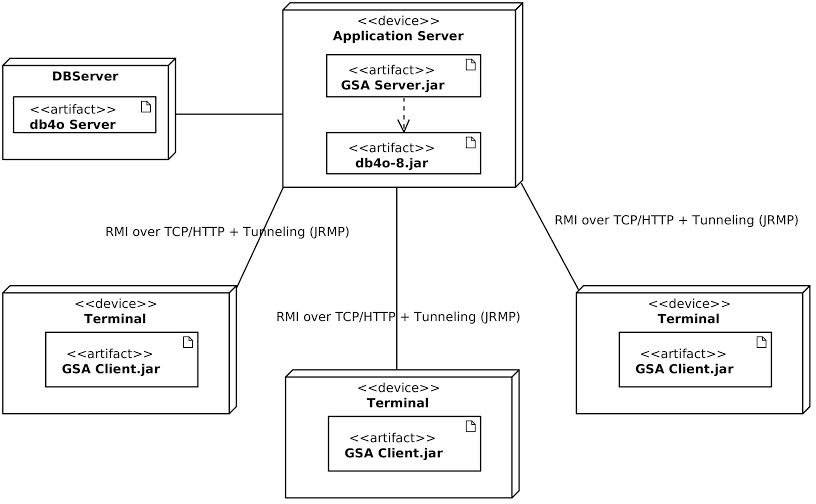
\includegraphics[width=\textwidth]{Deployment Diagram1.jpg}
\caption{Bozza dell'architettura di sistema}
\label{fig:deploy}
\end{figure}



 \section*{Interfacce}
 \subsection*{Hardware e interfacce significative}
Personal Computer installati in negozio.

Lettore laser per il codice a barre (normalmente sono collegati a una tastiera speciale, e l’input della scansione è considerata nel software come tasti premuti).

Stampante per le ricevute.

Stampante per le etichette (codice identificativo, prezzo, status se nuovo o usato) da applicare ai prodotti usati e/o nuovi (da definire).

Lettore di carte di credito o bancomat.

 \subsection*{Interfacce software}
Si prevedono interfacce Java, facenti uso delle librerie Swing, differenziate per cassieri, manager e Clienti, affinché soddisfino adeguatamente i compiti di ciascuno di essi.
 
 \section*{Regole di dominio (di business) specifiche dell'applicazione}
 \begin{tabular}{|p{.1\textwidth}|p{.4\textwidth}|p{.2\textwidth}|p{.2\textwidth}|}
 \hline
  \textbf{ID} & \textbf{Regola} & \textbf{Modificabilità} & \textbf{Sorgente} \\
  \hline
  BR1 &
  Con la tessera fedeltà il cliente ha diritto a sconti, indipendenti dalle promozioni temporanee. &
  In futuro il cliente potrà voler utilizzare i dispositivi mobili al posto della tessera, tramite la tecnologia NFC o QR-CODE. Semplicemente portando addosso un dispositivo con una applicazione dedicata. &
  La tecnologia si sta diffondendo e viene già adottata in molti scenari al posto di carte. Ad esempio pass di sicurezza.\\
  \hline
  BR2 & 
  Sono presenti sconti sui prodotti. &
  Gli sconti sono limitati nel tempo e dipendono da particolari eventi o periodi dell'anno. &
  È la politica di molti negozi.\\
  \hline
  BR3 &
  Sono proposti scambi tra prodotti usati e nuovi. &
  In determinati periodi sono presenti offerte di scambio, altamente suscettibili alle condizioni dei prodotti usati e al loro valore in quel determinato momento, inoltre sono specifiche per alcuni tipi di prodotto. &
  È la politica di alcune catene di videogiochi. \\
  \hline
  BR4 &
  Regole fiscali sulle imposte. Bisogna vedere leggi e regolamenti sulle imposte per prodotti usati e nuovi. &
  Elevata. Le imposte cambiano quasi ogni anno, vedasi aumenti dell'IVA. &
  Leggi nazionali.\\
  \hline
 \end{tabular}

\section*{Informazioni nei domini di interesse}

\subsection*{Determinazione del prezzo}
Oltre alle regole di determinazione del prezzo, presenti tra le regole di dominio, bisogna evidenziare che i prodotti usati vengono valutati in base a dei criteri, quali il prezzo dell'originale, la condizione, la richiesta del prodotto, ecc. 

\subsection*{Codici identificativi degli articoli}
Il Sistema GameShop Advance deve supportare diversi schemi di identificazione degli articoli (UPC, EAN, SKU). In alcuni casi i codici identificativi vengono generati direttamente dal sistema, in negozio. Particolare importanza riveste quindi il codice SKU (Stock Keeping Units) che sono codici identificativi definiti dal negoziante in modo completamente arbitrario.

\subsection*{Gestione dei pagamenti con carta di credito o} bancomat
Quando un pagamento elettronico con bancomat o carta di credito è stato approvato da un servizio di autorizzazione ai pagamenti, è quest’ultimo il responsabile del pagamento al venditore, non più l’acquirente. Di conseguenza, per ciascun pagamento il venditore deve registrare il denaro a lui dovuto tra i crediti da riscuotere dal servizio di autorizzazione.

\subsection*{Imposte sulle vendite}
Bisogna approfondire le conoscenze in tale ambito dato che il calcolo delle imposte può risultare complesso, poiché cambia regolarmente in conformità alle leggi. E’ pertanto consigliabile delegare il calcolo delle imposte a un calcolatore software prodotto da terzi.
\end{document}          
